
%%%
% Discussion of how each strategy was used as a separate starting point
%%%

\subsubsection*{Starting Points}
\label{sec:findings-expts-starts}

%%%
Since a desired outcome of the learning process was to be able to use the
generated strategy graphs to tell how a hand \textit{should} be played in a
certain score position,
a comparison was made between the produced agent and pure strategies
on a database of choices made by humans.
%
There exists a website in which users are prompted with a set of dealt cards and
a given score and must decide which set of cards they would keep in that
specific situation
\cite{dailycribbagehand}.
%%%

%%%
With access to recorded answers,
the agent's choices could be compared to how humans ranked the choice.
%
The retrieved database recorded which responses were given to each query
and could be used to determine how well the agent's choice matched with those
made by humans in the same situation.
%
For each of the more than 3600 usable records,
the choice the agent made was compared against those made by the users of the
website.
%
The results of this comparison can be seen in
Table~\ref{tab:expts-starts-human}. % TODO: ref more tables if created
%%%

%%%
Table~\ref{tab:expts-starts-human} shows that the trained agent chooses the same
set of cards as the human users only marginally more often than an agent with 
randomly allocated weights.
%
In approximately half of the cases,
the trained agent chooses the same answer as most humans;
in almost 78 percent of the cases,
the answer given by the agent is within the top three most common human answers.
%
Additionally,
most pure strategies,
created by setting their weight to 1 while all others are 0,
performed worse than the trained mixture.
%
Notable exceptions to this trend are the \handmaxposs\ and \handmaxavg\ 
strategies,
suggesting that in more situations than the agent,
the typical human player will play more according to what points can be expected
to be gained from the cut card.
%
Interestingly,
the \handmaxposs\ strategy's presence as the second most common pure strategy
used indicates a significant degree of risk-taking present in the users'
responses.
%%%

%%%
As a result of this finding,
each of these strategies were used as initial weights to the learning process
in order to determine if the agent could learn to fine-tune a policy starting
from a reasonable assertion of good game-play
as well as learn to discount demonstrably poor strategies.
%
Since the update mechanism for weights relies upon renormalization of a vector
which as been rewarded or punished,
no modifications would occur in the case of punishment of a pure strategy
since no other weights would have the chance to increase.
%
Therefore,
the pure strategies used before were slightly modified so that each other
element of the \wvec\ vector would have a small initial value which would be
increased when the pure strategy was punished.
%%%


\begin{table}

	\begin{tabular}{|r|c|c|c|p{4cm}|}
		\hline
		\textbf{Strategy} & \textbf{Top 1} & \textbf{Top 2} & \textbf{Top 3}
			& \textbf{Percentage in Top 3 Human Choices} \\
		\hline
		\peggingminavggiven & 160 & 303 & 458 & 12.64 \\\hline
		\peggingmaxmedgained & 268 & 519 & 796 & 21.97 \\\hline
		\peggingmaxavggained & 347 & 650 & 963 & 26.58 \\\hline
		\cribminavg & 380 & 177 & 1081 & 29.84 \\\hline
		\handmaxmin & 1576 & 2288 & 2666 & 73.59 \\\hline
		\textbf{Random} & \textbf{1581} & \textbf{2318} & \textbf{2759} &
			\textbf{76.15} \\\hline
		\handmaxmed & 1649 & 2353 & 2768 & 76.40 \\\hline
		\textbf{Trained} & \textbf{1706} & \textbf{2426} & \textbf{2821} &
			\textbf{77.86} \\\hline
		\handmaxposs & 1677 & 2433 & 2847 & 78.58 \\\hline
		\handmaxavg & 2066 & 2828 & 3168 & 87.44 \\\hline
	\end{tabular}
	% total = 3623
	\caption{
		Number of times the agent using a given strategy chose the same cards as
		the most common choice by human users
		according to 3623 total parsable records obtained from
		\cite{dailycribbagehand}.
		The columns labeled ``Top X'' display the number of times the given
		strategy's choice was within the top X choices of the user base.
		%if at least that many different choices were made
		In this table,
		\textbf{Random} is from the best result of five agents which each used
		independently randomly allocated weights
		and
		\textbf{Trained} uses an agent trained from Round 2 for one million
		games.
	}
	\label{tab:expts-starts-human}
\end{table}



\paragraph*{Results}

%%%
There are very two interesting trends that arise from starting from nearly pure
strategies.
%
The first is that the starting strategy is,
at least for those tested,
is the dominant strategy in winning positions.
%
Similarly,
this strategy is always un-learned in losing positions.
%
This serves as a confirmation that losing positions are simply unlikely to be
recovered from by the agent,
no matter how seemingly rational the strategy is.
%
There are two likely reasons for this dominance of the winning positions'
weights.
%
The first,
the pure mathematical operation of overcoming such an astoundingly heavily
weighted strategy requires many games to explore enough and perform better than
the given strategy
which itself may often coincide with \handmaxavg\ or \handmaxmin\ 
which would normally occupy these positions.
%
The second,
since the opponent is a static agent always using the same starting
mostly pure strategy and never training these weights,
playing a similar strategy ensures a similar resulting position.
%
When already in the lead,
this desirable as the agent will likely continue to be in a winning position
and closer to the goal score of 121.
%%%

%%%
An intriguing counter to this pattern of dominance in winning positions
is the \handmaxavg\ strategy
which yields some control of winning positions to \handmaxmed.
%
In normal training procedures,
this space is occupied by \handmaxmin.
%%%

%%%
The second interesting observation is what learning does occur
in the losing positions.
%
With most starting strategies,
the losing positions are mainly left to the influence of a single
other strategy.
%
This losing strategy also varies depending on the starting strategy.
%
The reason for this varying losing strategy is again
because the opponent for each of these agents during training
was an agent always using the same mostly pure strategy.
%
As a result,
the learning agent developed a counter strategy to each different
opponent it faced.
%
For instance,
when faced with \handmaxmin\ which will always play safe,
the agent learns to swing for the fences by playing according to \handmaxposs\ 
when it is losing
since the opponent will not be taking any risks itself
and risk is the only way to make up ground.
%
Similarly,
the agent learns that the best way to recover from a losing position
against \handmaxavg,
which plays to expectations and avoids unnecessary risk,
is to mostly play safely according to \handmaxmin.
%
As a counter to the dominance of a single strategy in the losing positions,
starting with \handmaxposs\ leads to a losing strategy
shared between \handmaxavg\ and \handmaxmed.
%
This is because either of these two strategies is likely to recover ground
against an agent which always tries to get the maximum amount of points
with no regard for the likelihood of this outcome.
%%%

% fig:findings-expts-sanitycheck-matrix
\begin{figure}
\centering

\begin{tabular}{ l l l l l l } %    c}
	%                    label
	%  l            | l1   l2   l3   l4
	%  a   ---------+-------------------
	%  b   starting | a1 | a2 | a3 | a4
	%  e   strat    | b1 | b2 | b3 | b4
	%  l   ...
	& & \multicolumn{4}{c}{\textit{Strategy}} \\
	& & \handmaxmin & \handmaxavg & \handmaxposs & \handmaxmed \\
	%\cline{3-6}
	\multirow{7}{*}{
	\rotatebox{90}{
	\parbox[c]{6.5cm}{
		\textit{Starting Strategy}
	}
	}
	}
	%
	& \rotatebox[origin=c]{90}{\handmaxmin}
		&\parbox[c]{1em}{
\includegraphics[width=2.5cm]{images/findings/experiments/starting_points/matrix_handmaxmin_handmaxmin.png}}
		&\parbox[c]{1em}{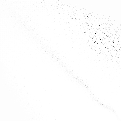
\includegraphics[width=2.5cm]{images/findings/experiments/starting_points/matrix_handmaxmin_handmaxavg.png}}
		&\parbox[c]{1em}{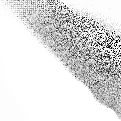
\includegraphics[width=2.5cm]{images/findings/experiments/starting_points/matrix_handmaxmin_handmaxposs.png}}
		&\parbox[c]{1em}{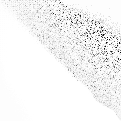
\includegraphics[width=2.5cm]{images/findings/experiments/starting_points/matrix_handmaxmin_handmaxmed.png}}
		%&
	\\ & & & & & \\
	%
	& \rotatebox[origin=c]{90}{\handmaxavg}
		&\parbox[c]{1em}{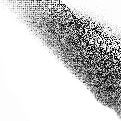
\includegraphics[width=2.5cm]{images/findings/experiments/starting_points/matrix_handmaxavg_handmaxmin.png}}
		&\parbox[c]{1em}{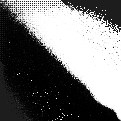
\includegraphics[width=2.5cm]{images/findings/experiments/starting_points/matrix_handmaxavg_handmaxavg.png}}
		&\parbox[c]{1em}{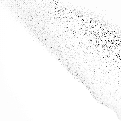
\includegraphics[width=2.5cm]{images/findings/experiments/starting_points/matrix_handmaxavg_handmaxposs.png}}
		&\parbox[c]{1em}{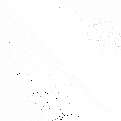
\includegraphics[width=2.5cm]{images/findings/experiments/starting_points/matrix_handmaxavg_handmaxmed.png}}
		%&\parbox[c]{1em}
	\\& & & & & \\
	%
	& \rotatebox[origin=c]{90}{\handmaxposs}
		&\parbox[c]{1em}{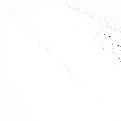
\includegraphics[width=2.5cm]{images/findings/experiments/starting_points/matrix_handmaxposs_handmaxmin.png}}
		&\parbox[c]{1em}{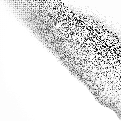
\includegraphics[width=2.5cm]{images/findings/experiments/starting_points/matrix_handmaxposs_handmaxavg.png}}
		&\parbox[c]{1em}{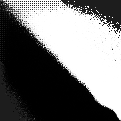
\includegraphics[width=2.5cm]{images/findings/experiments/starting_points/matrix_handmaxposs_handmaxposs.png}}
		&\parbox[c]{1em}{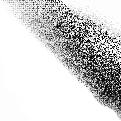
\includegraphics[width=2.5cm]{images/findings/experiments/starting_points/matrix_handmaxposs_handmaxmed.png}}
		%&\parbox[c]{1em}
	\\& & & & & \\
	%
	& \rotatebox[origin=c]{90}{\handmaxmed}
		&\parbox[c]{1em}{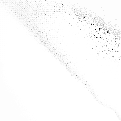
\includegraphics[width=2.5cm]{images/findings/experiments/starting_points/matrix_handmaxmed_handmaxmin.png}}
		&\parbox[c]{1em}{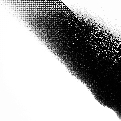
\includegraphics[width=2.5cm]{images/findings/experiments/starting_points/matrix_handmaxmed_handmaxavg.png}}
		&\parbox[c]{1em}{
\includegraphics[width=2.5cm]{images/findings/experiments/starting_points/matrix_handmaxmed_handmaxposs.png}}
		&\parbox[c]{1em}{
\includegraphics[width=2.5cm]{images/findings/experiments/starting_points/matrix_handmaxmed_handmaxmed.png}}
		%&\parbox[c]{1em}
	\\
\end{tabular}

\caption{}
\label{fig:findings-expts-sanitycheck-matrix}
\end{figure}


%%%
As this experiment showed promise in an agent potentially learning
to out-play its opponent,
an agent trained with a beginning pure strategy of \handmaxavg\ was played
against its previous iterations in several 10,000-game tournaments.
%
% TODO: vvv sanity check results
The results,
depicted in Figure~\ref{fig:expts-sanitycheck-spreads}
show that ... TODO ...
%%%

% fig:expts-sanitycheck-spreads[-{a,b}]
% Point spreads for two runs of blah

\begin{figure}
\center

% TODO: actual images

\begin{subfigure}[t]{0.45\textwidth}
	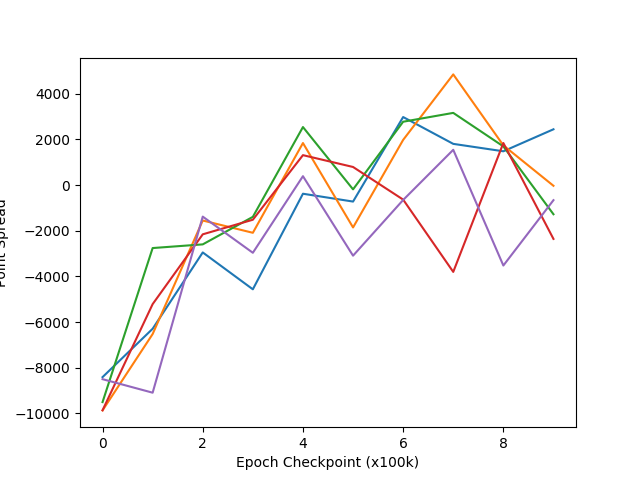
\includegraphics[width=\linewidth]{images/findings/experiments/starting_points/tourny_a.png}
	\caption{
		A trained agent starting from a semi-pure \handmaxavg\ strategy
		plays against previous iterations of itself.
	}
	\label{fig:expts-sanitycheck-spreads-a}
\end{subfigure}
~
\begin{subfigure}[t]{0.45\textwidth}
	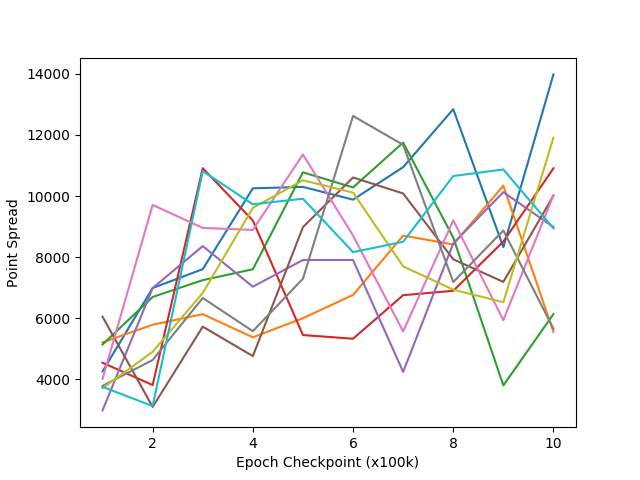
\includegraphics[width=\linewidth]{images/findings/experiments/starting_points/tourny_b.png}
	\caption{
		An agent using a semi-pure \handmaxavg\ strategy
		plays the epoch checkpoints of an agent which has been trained
		against this strategy.
	}
	\label{fig:expts-sanitycheck-spreads-b}
\end{subfigure}

\caption{
	Point spreads of several 10,000-game tournaments
	between agents of varying training levels
	when started with set of semi-pure \handmaxavg\ strategy weights.
}
\label{fig:expts-sanitycheck-spreads}
\end{figure}


%%%
% TODO: vvv sanity check second training round results
Furthermore,
as the agents were previously each trained against different pure strategies,
the ability to improve a basic policy to overcome a randomly-weighted agent,
rather than to learn a policy from scratch,
was tested by training an agent starting with a semi-pure
\handmaxavg\ strategy against an unlearning agent with random weights.
%
The results of this further training,
seen in Figure~\ref{fig:expts-sanitycheck-strats},
show that ... TODO ...
%%%

% fig:expts-sanitycheck-strats

\begin{figure}
\center

% TODO: actual images

	\begin{subfigure}[t]{0.22\textwidth}
		%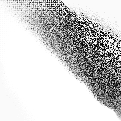
\includegraphics[width=\textwidth]{images/findings/experiments/starting_points/hand_max_min.png}
		\caption{\handmaxmin}
	\end{subfigure}
	~
	\begin{subfigure}[t]{0.22\textwidth}
		%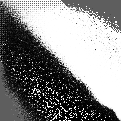
\includegraphics[width=\textwidth]{images/findings/experiments/starting_points/hand_max_avg.png}
		\caption{\handmaxavg}
	\end{subfigure}
	~
	\begin{subfigure}[t]{0.22\textwidth}
		%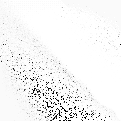
\includegraphics[width=\textwidth]{images/findings/experiments/starting_points/hand_max_med.png}
		\caption{\handmaxmed}
	\end{subfigure}
	~
	\begin{subfigure}[t]{0.22\textwidth}
		%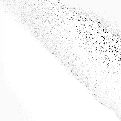
\includegraphics[width=\textwidth]{images/findings/experiments/starting_points/hand_max_poss.png}
		\caption{\handmaxposs}
	\end{subfigure}

	\begin{subfigure}[t]{0.22\textwidth}
		%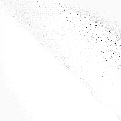
\includegraphics[width=\textwidth]{images/findings/experiments/starting_points/crib_min_avg.png}
		\caption{\cribminavg}
	\end{subfigure}
	~
	\begin{subfigure}[t]{0.22\textwidth}
		%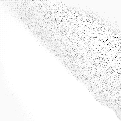
\includegraphics[width=\textwidth]{images/findings/experiments/starting_points/pegging_max_avg_gained.png}
		\caption{\peggingmaxavggained}
	\end{subfigure}
	~
	\begin{subfigure}[t]{0.22\textwidth}
		%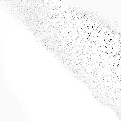
\includegraphics[width=\textwidth]{images/findings/experiments/starting_points/pegging_max_med_gained.png}
		\caption{\peggingmaxmedgained}
	\end{subfigure}
	~
	\begin{subfigure}[t]{0.22\textwidth}
		%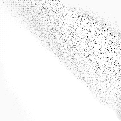
\includegraphics[width=\textwidth]{images/findings/experiments/starting_points/pegging_min_avg_given.png}
		\caption{\peggingminavggiven}
	\end{subfigure}

\caption{
	All final strategy strengths for an agent
	which started with a 70\% semi-pure \handmaxavg\ strategy
	and was trained against an agent with unchanging random weights
	for one million games
	when playing as the dealer.
}
\label{fig:expts-sanitycheck-strats}
\end{figure}


